\part{System design}
\chapter{System design}

In this chapter, component selection and design is described.

During the design process, multiple iteration of component selection, validation and link budget calculation were made, this chapter describes the final result of the link design. 

\section{Space segment}
Space segment is a part of the satellite communication system that resides on the satellite itself. It is divided into two main parts: communication subsystem (COMM) and antennas (ANTs) connected with two coaxial cables.

Space segment is critical in system operation and reliability - there is no possibility to carry out any repairs. It is exposed to the space environment - thermal cycling, cosmic radiation and vacuum.

Because of the mentioned requirements it was decided to choose commercially available and flight-proven Cubesat components to increase the reliability of the system.

\subsection{Frequency band selection}
Data throughput requirements and communication session scheme were described in the \ref{introduction} chapter, but it summarizes to about \SI{1}{\kbps}.

As mentioned in section \ref{aa} the most common radio bands used in Cubesat designs are VHF, UHF and S-band. S-band is usually used when high data rate (~\SI{10}{\Mbps}) are necessary. Typical designs for low-rate data link are full-duplex combo or simplex VHF/UHF radio.

PW-Sat1 (first polish satellite, built on Warsaw University of Technology) - (link)??? used full-duplex VHF-downlink and UHF-uplink radio. During its mission, uplink stability was an issue. The cause was narrowed down to very high level of noise and interference in the UHF band on the orbit, which probably is caused by over-the-horizon radars. Therefore, UHF-uplink was discarded.

Concluding, the selected band for operation were either simplex VHF or VHF-up, UHF-down full-duplex.

\subsection{Communication subsystem}
Communication subsystem of the satellite is responsible of transmitting and receiving radio signals, modulating/demodulating them and providing data link for the On Board Computer. It has to be compatible with selected mechanical configuration, available data interfaces and the antennas to be installed.

Cubesat standard, with which PW-Sat2 is compliant, defines PC/104 connector, which is the main data bus for all satellite subsystems. Radio should use \iic bus to send and receive data from the on-board computer.

When the subsystem was ordered, the choice of available products was very limited, and the only radio which was compliant with above mentioned requirements was \texttt{ISIS VHF uplink/UHF downlink Full Duplex Transceiver}. Its view and block diagram is shown in the figure \ref{ISIS_TRXvU}

\begin{figure*}
   \centering
\begin{tabular}{cc}
        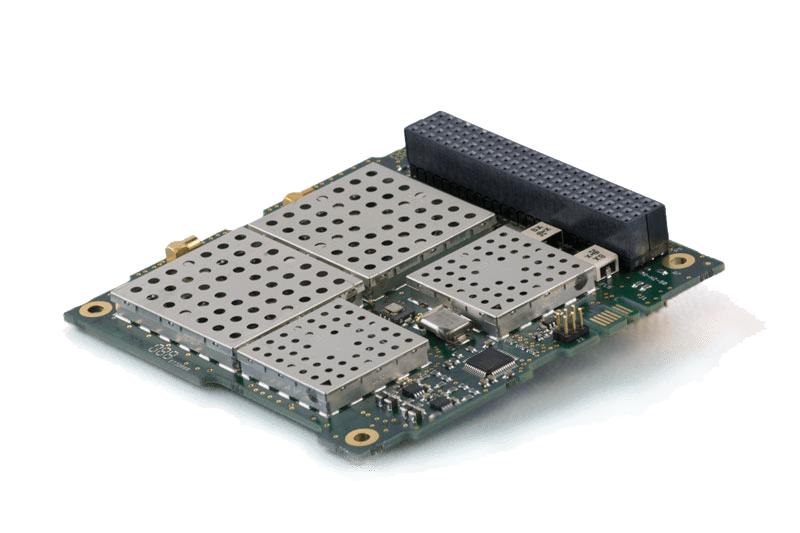
\includegraphics[width=0.4\paperwidth]{img/2/ISIS-radio-UHF-VHF-min.png}
    & 
        %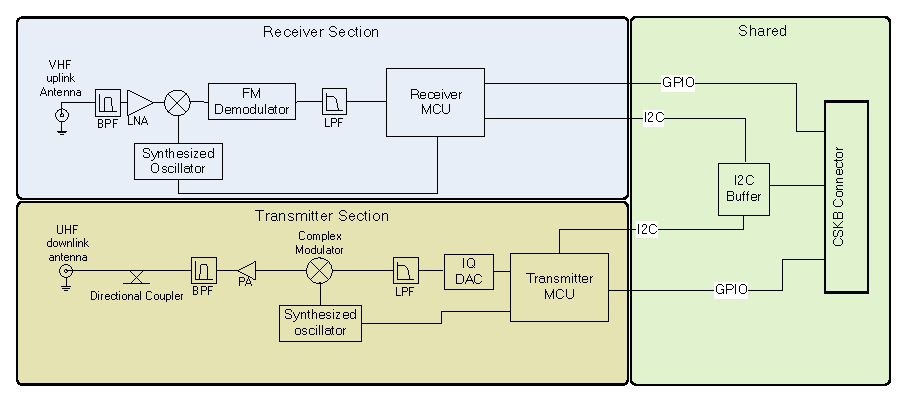
\includegraphics[width=0.3\paperwidth]{img/2/ISIS_TRXvU_block_diagram.eps}
\end{tabular}
\label{ISIS_TRXvU}
\caption{ISIS VHF uplink/UHF downlink Full Duplex Transceiver. Source: \cite{???}}
%%% https://www.isispace.nl/product/isis-uhf-downlink-vhf-uplink-full-duplex-transceiver/
\end{figure*}

Basic characteristics:

\begin{tabular}{c|c}
     \textbf{downlink} & \textbf{uplink} \\ \hline
     \multicolumn{2}{c}{dual-\iic communication standard} \\
     \multicolumn{2}{c}{AX.25 frame format} \\
     \si{430}-\SI{450}{\MHz} frequency range & \si{140}-\SI{150}{\MHz} frequency range \\
     \SI{0.5}{\watt} downlink power & \SI{-98}{\dBm} sensitivity for \si{10^-5}~BER \\
     \si{1.2} - \SI{9.6}{\kilo\bit / \second} bitrate & \SI{1.2}{\kilo\bit / \second} bitrate \\ 
     BPSK modulation with G3RUH scrambling & FM-modulated AFSK \\ 
\end{tabular}



\subsection{Antennas}
Because of the selected radio system, two antennas has to be installed - one for uplink (VHF) and one for downlink (UHF).

Antennas for this frequencies has to be larger than CubeSat structure - hence  they have to be deployed after release from launcher vehicle. They should be omnidirectional, as PW-Sat2 does not have a pointing possibility and random tumbling is assumed. Typically satellites operate with circular polarization (this is favorable due to satellite rotation), but due to size and weight constraints antenna can have linear polarization.

The most simple antenna for this purpose would be monopole or dipole. Dipole antenna would be more stable in changing objects around - as the PW-Sat will deploy its solar panels and deorbit sail.

Self - made dipole was considered at the design stage, but due to mechanical and time constraints, satellite antenna was decided to be bought. Along with the transceiver, ISIS company does manufacture compatible and tuned antennas for their communication modules. \texttt{CubeSat dipole antenna system} was selected.

This system is deployable by the command from on-board computer. Thermal knife (resistor) is heated up and thermal link is burnt, resulting is antenna deploy by spring action. Antenna is shown in the figure \ref{ISIS_antenna}.

%% TODO: znaleźć zdjęcie złożonej anteny i zmergować
    \begin{figure}[H]
        \centering
        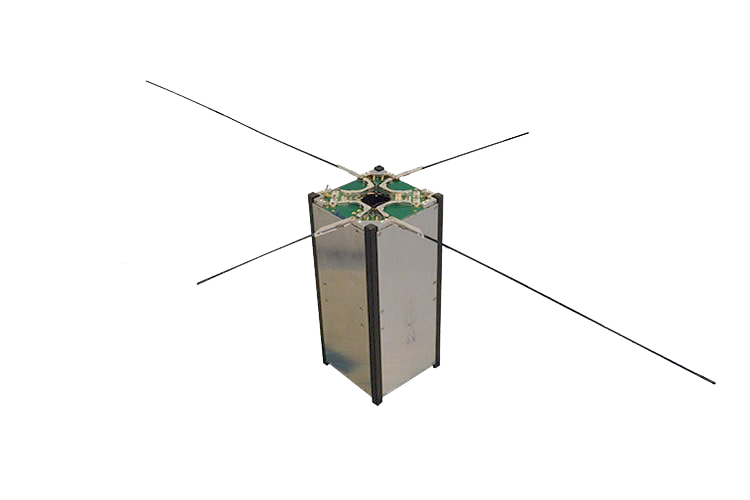
\includegraphics[width=0.8\paperwidth]{img/2/CubeSat-antenna-dipole-configuration.png}
        \caption{ISIS CubeSat dipole antenna system. Source: \cite{???}}
        %%% https://www.isispace.nl/product/dipole-antenna-system/
        \label{ISIS_antenna}
    \end{figure}


\subsubsection{Deployable elements influence on the antenna pattern}

On-board PW-Sat2 are two main deployables: solar panels and deorbitation sail.

During design stage, influence of the solar panels was discussed with antenna manufacturer - the outcome was to place longed dipoles (VHF) along the solar panels, and shorter ones orthogonally to it, as shown in the figure \ref{???}

% TODO: zdjęcie z otwartymi panelami i antenami

The influence of the deorbit sail was also simulated during Critical Design stage.

Deorbitation sail is made by very thin (\SI{5}{\micro\meter}) mylar foil with aluminium coating. Using % TODO
simulation tool, it was shown that the sail will increase directivity of the cubesat antennas, acting as a reflector.
% TODO: jakieś zdjęcie z symulacji, wynik o ile dB się pogorszyło


\section{Communication link parameters}
Selected satellite radio module imposes the modulation and data packets used in the communication. This section briefly describes used modulations, frame formats and implications to the ground segment of the system.

\subsection{Downlink modulation}
Downlink signal is modulated using Binary Phase Shift Keying (BPSK). The data rate can be changed dynamically by the on-board computer, in range \si{1.2} - \SI{9.6}{\kilo\bit / \second}, allowing to improve the link quality when necessary. Baseband signal is also filtered using Raised Root Cosine filter, to reduce side lobes power. Signal bandwidth varies between \SI{2.4}{\kHz} (for \SI{1.2}{\kbps}) and \SI{19.2}{\kHz} (for \SI{9.6}{\kbps}). 

% TODO: rysunek BPSK

\subsection{Uplink}
Uplink modulation is two-staged: first, data is modulated using Audio Frequency Shift Keying (chaning 0s and 1s to wave of frequencies, in order, \SI{1200}{\hertz} and \SI{2200}{\hertz}), later to be Frequency Modulated to the RF carrier (with frequency deviation of $\pm\SI{5}{\kilo\hertz}$).

% TODO: schemat modulatora

\subsection{Frame format}
Physical layer data format is reduced-functionality AX.25 packet \cite{AX25_standard}. Only connectionless transmission mode and UI frames are supported. Packet framing is the same as in SwissCube CubeSat \cite{SwissCube_AX25}.

Basic frame format is shown in the table \ref{AX25_frame}. All the fields except flags are bit-stuffed to ensure that the \textit{Flag} field does not appear in the data: if there are six '1' bits to be send, transmitter inserts '0' bit before the last one. Adressing in this system in inherent, but unused - this is point-to-point connection, therefore adresses are fixed. Frame-Check Sequence is a CRC (CITT standard) of the whole frame (without \textit{Flags}). \textit{Information Field} is variable-length, between \si{4} and \SI{256}{\byte} length is the place for the actual data transmitted by the On-Board Computer.

\begin{table}
\small
\centering
\caption{AX.25 frame format}
\label{AX25_frame}
\arrayrulecolor{black}
\begin{tabular}{l|c|c|c|c|c|c|c|c|} 
\hhline{~|-|----|-|-|-|}
\multirow{2}{*}{}                                                              & \multirow{2}{*}{Flag } & \multicolumn{4}{c|}{AX.25 Transfer Frame Header (128 bits)}                                                                                                                                                                                   & {\cellcolor[rgb]{0.753,0.753,0.753}}                                                                                                                  & \multirow{2}{*}{\begin{tabular}[c]{@{}c@{}}Frame-\\Check\\Sequence\end{tabular}} & \multirow{2}{*}{Flag}  \\ 
\hhline{~|~|-|-|-|-|>{\arrayrulecolor[rgb]{0.753,0.753,0.753}}->{\arrayrulecolor{black}}|~|~|}
                                                                               &                        & \begin{tabular}[c]{@{}c@{}}Destination\\Address\end{tabular} & \begin{tabular}[c]{@{}c@{}}Source\\Address\end{tabular} & \begin{tabular}[c]{@{}c@{}}Control\\Bits\end{tabular} & \begin{tabular}[c]{@{}c@{}}Protocol\\Identifier\end{tabular} & \multirow{-2}{*}{{\cellcolor[rgb]{0.753,0.753,0.753}}\begin{tabular}[c]{@{}>{\cellcolor[rgb]{0.753,0.753,0.753}}c@{}}Information\\Field\end{tabular}} &                                                                                  &                        \\ 
\hline
\multicolumn{1}{|c|}{\begin{tabular}[c]{@{}c@{}}Length\\{[}bits]\end{tabular}} & 8                      & 56                                                           & 56                                                      & 8                                                     & 8                                                            & {\cellcolor[rgb]{0.753,0.753,0.753}}32-2048                                                                                                           & 16                                                                               & 8                      \\ 
\hline
\multicolumn{1}{|c|}{Value}                                                    & 01111110               & PWSAT2-0                                                     & PWSAT2-0                                                & 00000011                                              & 11110000                                                     & {\cellcolor[rgb]{0.753,0.753,0.753}}                                                                                                                  & CRC-CITT                                                                         & 01111110               \\
\hline
\end{tabular}
\end{table}


Additionally, downlink data is scrambled using G3RUH scrambling polynomial to maximize randomness and ensure proper bit synchronization.

%% -------------------------------------------------------------------------------------------

\section{Ground station design}
Ground station design should complement the space segment, with large antenna gains and output power to allow the budget link to close.

As the system is full-duplex, both uplink and downlink channels are separate.

\subsection{Antennas}
Space communication antennas require very large gain due to the distance between the stations. 

Typical design consist of two Yagi-Uda antennas, one for uplink (VHF) and one for downlink (UHF). Their length, therefore directivity was constrained by available space, antenna mast height, antenna rotator strength and positioning accuracy.

PW-Sat2 is transmitting radio signals with linear polarization, nevertheless ground station  polarization should be circular, due to the random tumbling of the satellite. To achieve this, Cross-Yagi antennas were selected, and two linear planes antennas were phased using coaxial cable and symmetrical splitters/combiners. Coaxial cables length was calculated to achieve \SI{90}{\degree} shift between two dipols.

% TODO: schemat anten w GS

Antennas were selected to be the longest possible, limited by mast height. I turned out that they are one of the longest commercially available. 

Antenna characteristics:

\begin{tabular}{c|c}
     \textbf{Downlink} & \textbf{Uplink} \\ \hline
     Tonna & Tonna \\
\end{tabular}


\subsection{Uplink}
Due to the low sensitivity of the satellite receiver (\SI{-98}{\dBm}) uplink EIRP has to be very large.
\subsubsection{Transmitter}
Uplink signal is an FM-modulated AFSK, so standard analog audio FM transceiver can be used to generate RF signal. Audio signal can be generated by the Terminal Node Controller or by software running on the PC.

During PW-Sat1 project, the Icom 910H amateur radio transceiver \ref{Icom_910H_ref} was used for both uplink and downlink, therefore it was proposed to use the the same radio.

\begin{figure}[H]
    \centering
    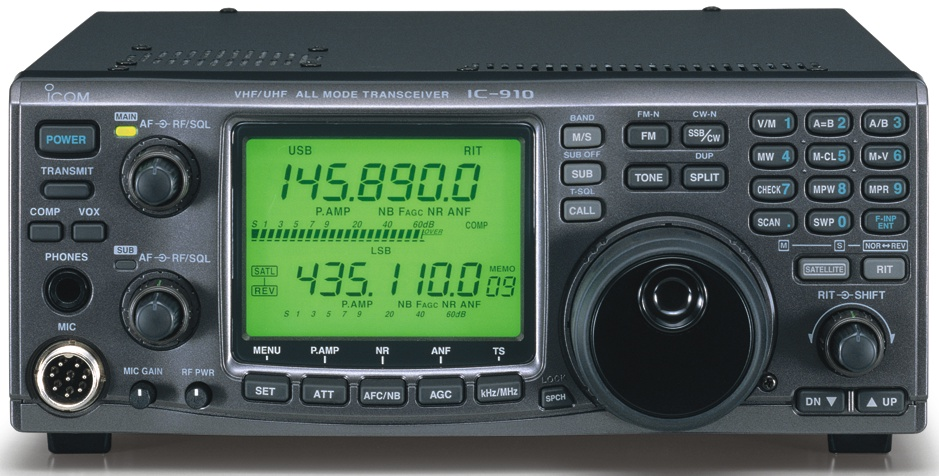
\includegraphics[width=0.6\paperwidth]{img/2/icom910h.jpg}
    \caption{Icom 910H. Source: \cite{ICOM_910H_pic}}
    %%% https://www.isispace.nl/product/dipole-antenna-system/
    \label{Icom_910H_ref}
\end{figure}

Radio VHF FM transmit characteristics:

\begin{tabular}{c|c}
    Frequency & \si{144} - \SI{148}{\MHz} \\
    Frequency stability &  \SI{\pm 3}{\ppm} \\
    Output power & \SI{100}{\watt} \\
    Audio input & analog jack \\
\end{tabular}

This radio is connected to the computer, which controls the audio to transmit and Push-To-Talk (PTT, transmission enable) signal. 

\subsubsection{Standing Wave Ratio meter}
To check proper antenna connection and ensure long-term monitoring a SWR (Standing Wave Ratio) meter should be installed. This instrument measures ratio of reflected power, thus providing information about antenna impedance matching.

% TODO: zdjęcie/zrzut z kamerki SWR metera



% ------------------------------------------------------------
% ------------------------- DOWNLINK -------------------------
% ------------------------------------------------------------

\subsection{Downlink}
Receiving Signals from maximal range of about \SI{3000}{\kilo\meter} from a \SI{0.5}{\watt} transmitter requires very high processing gain and low noise factor of the system. Another factor to take into account is Doppler effect, which has to be taken into account. On UHF frequencies, it reaches up to about \SI{15}{\kHz}.

\subsubsection{Signal front-end processing}
First stage processing has two main purposes - to lower the system noise (amplify the signal) and eliminate intermodulation (filtering).

Downlink system block diagram is shown in the figure \ref{Downln}.

% TODO SCHEMAT DOWNLINKU

Amplifier, installed close to the antenna reduces influence of the long cable to the receiver, reducing total system noise factor. However, strong signals in the proximity of the signal can be intermodulated in the LNA, resulting in variety of issues: from reduced gain to completely distorted signal.

As an amplifier, a high-level Low Noise Amplifier Mini-Circuits PGA-103+ was used, with additional SAW filter to reduce unwanted signals. Schematic and pcb layout of the designed board are shown in the figure \ref{LNA}

% TODO: LNA

Narrowband filter should be installed before the LNA. However, this requires the filter to have the lower loss possible, as the in-band loss in the filter directly affects noise figure of the system. For this purpose, cavity filter was selected. This, reasonably narrow band filter (\SI{1}{\MHz}), has very low insertion loss ($<$\SI{1}{\dB}).

Front-end signal processing was installed as close to the antenna as possible \ref{elka_skrzynka}.

% TODO: elka_skrzynka



To receive BPSK signals, radio amateurs commonly use transceiver with Single SideBand  (SSB) mode. In this mode radio acts as a multi-stage down-converter, allowing to receive baseband with audio card from PC. However, due to audio main purpose, typical radios have a bandpass filters about \SI{3}{\kHz} wide, effectively blocking wider transmissions. Using SSB mode for receiving PW-Sat2 is possible, however only for \SI{1.2}{\kbps} bitrate.

Another options of BPSK receiver is to use integrated transceiver in one chip. This solution is not possible for this system, as no off-the-shelf chips provide AX.25 support.

The proposed receiver so



\section{Ground support software}
Due to the Software-Defined Radio based architecture, apart from typical frame processing chain, additional software related to modulation and de-modulation is required.

There are multiple signal processing toolboxes to simplify digital signal processing, such as Matlab/Octave \cite{Matlab}, SciPy \cite{Scipy} and GNUradio \cite{Gnuradio}. GNUradio however, simplifies connecting to physical hardware and programming, by allowing to integrate system in block diagrams.

\subsection{GNUradio}
% TODO

\subsection{Data flow chain}
Basic assumption of the data flow was to separate frame building (byte-oriented) from signal processing (sample-oriented). Frame building was written in Python, whereas signal processing was built using GNUradio blocks and self-written custom out-of-tree modules. Communication between the layers was implemented using ZeroMQ asynchronous messaging library. Data flow is shown in the figure \ref{data_flow}.

% TODO: data_flow


\subsection{Uplink}
Uplink baseband signal (AFSK) has generated, to be later FM-modulated and transmitted using conventional radio.

AFSK signal was generated using software Voltage Controlled Oscillator (VCO), by generating tone (\si{1200} or \SI{2200}{\hertz}) according to the bit value (\si{0} or \si{1}, respectively).  Block diagram of the uplink modulator is shown in the figure \ref{uplink_block}.


\subsection{Downlink}
The aim of the downlink module is to fully process incoming IQ data from SDR to baseband data (frames).




\subsection{Satellite operation}

